\section{Motion Control}
Motivation, General idea, terminology, 
\subsection{Space Time Constraint}
\subsection{Optimal Control}
\subsection{Reinforcement Learning}

\section{Motivation}

A large variety of soft body animals live on our planet. Some examples of
such creatures are slugs, starfish, earthworms, octopus, and jellyfish. These
animals move in interesting ways due to their flexible body shapes and lack of
skeleton support. In this chapter we present a method of animating soft body characters, that
is, characters that do not have a skeleton.  In particular, our emphasis
is on creating animations of soft body creature locomotion, including
crawling, walking, rolling and jumping.  
Many hand-drawn animated characters move in such a flexible
manner that they seem to be boneless.  The animation principle of
\emph{squash-and-stretch} can be seen in its purest form with soft body
characters. In addition, as exemplified by our own tongues, even animals with
skeletons can have body parts that move without the help of
bones.  Our research is driven by the intellectual challenge of
simulating the locomotion of such soft body creatures, without resorting
to any form of rigid elements in our models.

There are two key aspects of anatomy that allow real soft-bodied creatures
to move: volume preservation and muscle contractions.  Our animation
system makes use of these same principles.  Soft body tissue is volume
preserving, due primarily to the incompressible nature of water.  This
volume preservation puts constraints on the degree of deformation that a
soft body may undergo.  We use volume-preserving finite elements to match
this aspect of soft body tissue.  The second important aspect of soft body
creatures is that they control the shape of their body by the contraction of
muscles.  If such a creature shortens only the muscles that run down the
right side of its body, this will cause the creature to bend towards the
right.  Note that volume preservation and muscle contractions often work
in concert to produce motion.  If a cylindrical creature uses radial
muscle contraction to make itself thinner, then the constraint of volume
preservation means that at the same time the creature will stretch
lengthwise.

Each of our soft body characters is represented as a tetrahedral mesh and
simulated using the finite element method. Our models typically contain
hundreds of tetrahedral elements, and controlling such a high degree of
freedom model poses a challenge.  The aforementioned muscles from real
animals provide a way of reducing the degrees of freedom in our
characters.  In addition to the tet mesh, each of our characters is
augmented with a collection of polyline paths, each of which represents a
muscle fiber.  A character changes its body shape by contracting these
muscle fibers, and this induces a shape change in the collection of tetrahedra
near the fibers. In theory, such a character could be controlled by
specifying the timing of various muscle contractions. However, unlike
controlling articulated figures using joint torques, the complex interplay
between muscles and soft body shapes makes the control problem exceedingly
challenging; even bending a limb of a soft body creature is much more
difficult than bending a joint of an articulated figure. For these
reasons, we decided that controlling a soft body creature by specifying
the changes to each muscle fiber would be a tedious method of control.

Our system provides a collection of intuitive controls for soft body
creature motion, such as moving a point of the character to a given
position, or regulating the character's linear or angular momentum. With this
collection of intuitive controls, we are able to animate a variety of
soft body characters, and in particular, we can demonstrate a wide array
of locomotion methods.  To move a character, we specify a set of
high-level goals (possibly time-varying), and these goals are turned into
an objective function that is passed to our solver.  For each time
step, we formulate and solve a constrained optimization problem, and this
gives us new muscle lengths.  These muscle lengths induce changes in
stress that are applied to the tetrahedral elements, and we then use our
physics simulator to advance the system forward in time.

An important part of our constraint solver is contact planning, and
this proves to be a challenge for soft bodies.  At each time step, our
solver must be able to predict how a change to the muscle contractions
will influence the points of contact between the character and the
ground.  For articulated figures, most optimization-based controllers assume that each point
of contact is static, which makes contact resolution relatively
straightforward to solve.  In our system, we cannot assume static
contact because sliding and breaking contact turn out to be quite
important strategies to control soft characters.  For instance, a soft
creature may need to widen its base in order to balance, and this
means that the points of contact must slide.  Depending on the motion
goals that are given for a character, the best way to minimize the
resulting objective function might be to maintain static contact, to
break contact, or to allow sliding contact along the ground.  The
behavior needs to be decided for each point of contact, and this
results in a high dimensional and discontinuous optimization problem.  We formulate this
as a linear complementarity problem with a quadratic objective
function.  Although similar problems have been recently proposed in
other fields~\cite{Braun:2005,Bai:2011}, we believe that our solution method is new to
graphics.

A natural alternative to our approach would be to represent a character as
a rigid, articulated skeleton, and to surround the skeleton with soft
tissue that deforms.  Such a character representation could even
demonstrate elongation and contraction with the use of translational
joints.  This approach would have several advantages, including the
availability of numerous tools that can be used to control an articulated
figure.  We made a deliberate choice to avoid using rigid elements
entirely.  We think that using only soft elements will be more likely to
result in motions that are more faithful to actual soft body creatures.
Our approach avoids the possibility that the character motion shows hints
of a hidden skeleton.  In addition, using only muscle contractions keeps
our character motions ``honest'' in terms of the magnitude of forces that
such characters can apply without a skeleton.  Perhaps the most important
reason that we avoid the use of rigid elements is our desire to expand the
creature body forms that we can simulate using computers.  Many animals in
nature move without the use of skeletons, so is it possible to create a
computer simulation that mirrors this fascinating phenomenon?

\section{System Overview}

\begin{figure}[ht]
  \centering
  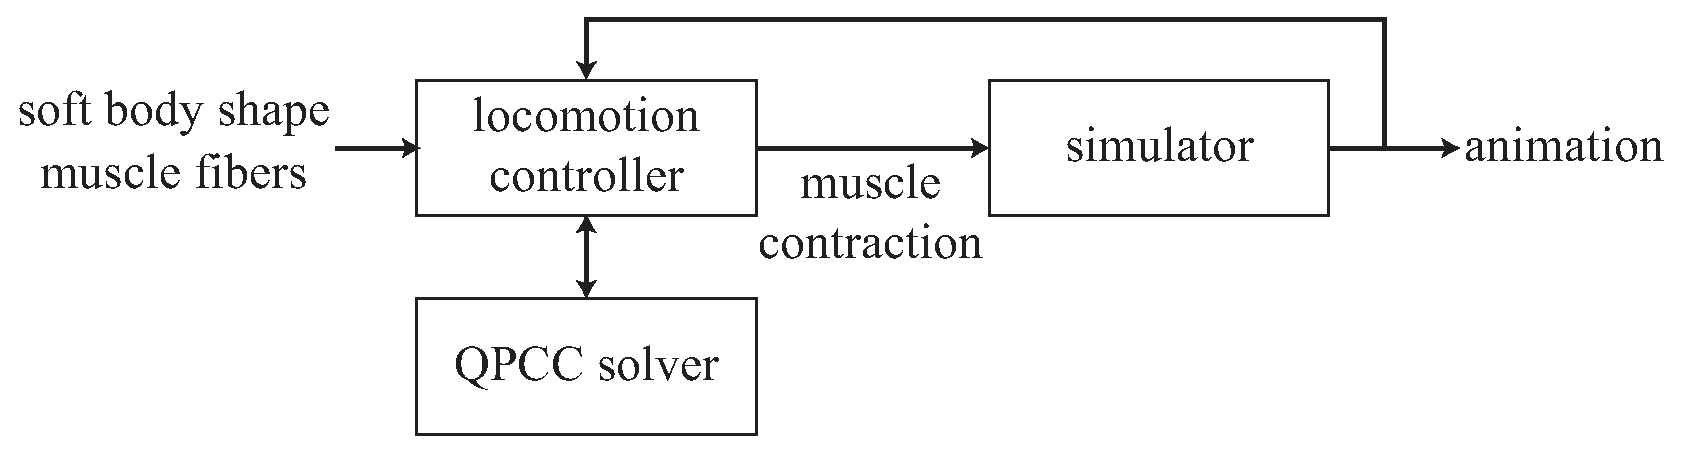
\includegraphics[width=5in]{figures/overview3}
  \caption{Overview of our system.}
  \label{fig:overview}
\end{figure}

We design a wide variety of locomotion controllers for soft bodies,
including balance, walking, crawling, jumping, sliding and rolling.
Given the geometry of a soft-body creature and the
arrangement of its muscle fibers, our controller computes required
muscle contraction to propel the creature to achieve desired
locomotion while maintaining balance. At each time step, the
controller formulates a quadratic program with complementarity
constraints (QPCC) to solve for the optimal muscle contraction under
discretized dynamic equations of motion and frictional contact
constraints. The objective function, assuming a convex quadratic form,
can be designed arbitrarily to address control goals of the desired
locomotion. The optimal muscle contraction is passed to a FEM
simulator to calculate the next state. Figure \ref{fig:overview}
illustrates the main components of our system.

\section{Soft Body Simulation and Modeling}
Before we introduce the control algorithms for locomotion, we first
describe the methods for simulating soft bodies and computing muscle
forces.

\subsection{Finite Element Simulation}
A soft body creature is represented as a tetrahedral mesh and
is simulated using a modified corotational linear FEM
\cite{Muller:2002}. We chose FEM instead of a mass-spring model
because it is difficult to enforce volume preservation for the material with mass-spring systems.
At each time step, the state of the creature,
$\vc{p}$, is computed through numerical integration of the dynamic
equations of motion:
\begin{equation}
\vc{M}\ddot{\vc{p}} = \vc{f}_{x} + \vc{f}_{e}+\vc{f}_{d}+\vc{f}_{m}
\label{eq:softDynamics}
\end{equation}
where $\vc{M}$ is the mass matrix of the discretized soft body and
$\vc{p}$ is the nodal position of the deformed shape. The forces on
the right hand side, $\vc{f}_{x}$, $\vc{f}_{e}$, $\vc{f}_{d}$, and
$\vc{f}_{m}$, indicate external, elastic, damping, and muscle forces
respectively. The external force $\vc{f}_{x}$ includes gravity,
contact force, and user perturbation force.

As notation, when we are specifying a quantity $\vc{q}$
for a single element, we will write this as $\hat{\vc{q}}$.
To compute the elastic force for each element, we adapted the method
suggested by Nesme \etal \cite{NPF05}:
\begin{equation}
\hat{\vc{f}}_e=-\hat{\vc{B}}^T\hat{\vc{D}}\hat{\vc{B}}(\hat{\vc{p}}-\hat{\vc{R}}\hat{\vc{x}})
\end{equation}
where $\hat{\vc{x}}$ indicates the nodal position in the rest shape
and $\hat{\vc{R}}$ transforms the element from the reference
coordinates to the deformed coordinates. $\hat{\vc{B}}$ is the
strain-displacement matrix in the deformed coordinates
and $\hat{\vc{D}}$ is the stress-strain matrix. We use the Poisson ratio 0.45 in $\hat{\vc{D}}$ to make the soft body
nearly incompressible while avoiding locking artifacts \cite{Irving:2007}. Although volume preservation is not enforced strictly, our experiments show that the volume change is below 15\% and is not visually noticeable.
This formulation linearizes the
elastic force around the current deformed shape, rather than around
the rest shape, as used in most FEM implementations. We chose this
formulation because it eliminates ``ghost torques'' caused by the
error of linearization around the rest shape~\cite{NPF05}. When the material is soft or when the deformation is
small, ghost torques do not cause visible artifacts. However, this
formulation is necessary for our case, because soft body locomotion
requires large deformation with relatively stiff materials to support
the weight of the creature.

We assemble the individual stiffness matrices $\hat{\vc{B}}^T\hat{\vc{D}}\hat{\vc{B}}$ for
each element into a large stiffness matrix $\vc{K}$ for the whole
system. The elastic force for all the FEM nodes can be expressed by
$\vc{f}_e=-\vc{K}(\vc{p}-\vc{R}\vc{x})$. For damping force, we use
simple Rayleigh damping model to compute its effect:
$\vc{f}_d=-\vc{C}\dot{\vc{p}}=-(\mu\vc{M}+\lambda\vc{K})\vc{\dot{p}}$. We
set $\mu = 0$ and $\lambda = 0.2$.

\subsection{Muscle Modeling}
We model muscle fibers as polygonal curves with a small number of
segments. Each muscle segment can contract along its current direction, but
it cannot extend or bend. Based on the arrangement of muscle fibers,
we can bundle them into muscle groups. There are three types of
muscles which lead to different control tasks. The \emph{longitudinal
muscles} are linear muscles that extend from one end of the body to the
other end. Their main function is to shorten or bend the body. The
\emph{radial muscles} are a set of short muscles that span a cross-section
of the body. When radial muscles contract, the volume-preserving
nature of the tissue causes the body to elongate. \emph{Helical
muscles} wrap around the body in a helical shape. When a helical muscle
contracts, the body twists.

\ignorethis{These three types of muscles are found in
a variety of soft body creatures and deformable body parts
\cite{Kier:1985}, including worms, elephant trunks, squid tentacles
and human's tongues.}

Muscle contraction induces muscle force on nearby FEM elements. Each
muscle segment is modeled as a spring with a changeable desired
length. The spring force caused by each segment is computed as: $f =
k(l_d - l)$, where $k$ is the stiffness of the muscle fiber, $l_d$ is
the current desired length, and $l$ is the current length of the
segment. We treat $f$ as a virtual force, which is realized by muscle
stress imposed on nearby elements. When a muscle segment contracts
with the virtual force $f$ in the direction of $\vc{d}$ in the
reference coordinates, the effect of contraction is as muscle
stress $\vc{F}$:
\begin{equation}
\vc{F}=\vc{U}\left[\begin{array}{ccc}
f & 0 & 0\\
0 & 0 & 0\\
0 & 0 & 0
\end{array}\right]\vc{U}^T
\end{equation}
where $\vc{U}$ is the matrix that rotates vector $(1, 0, 0)^T$ in the
reference coordinates to be aligned with $\vc{d}$.

Each FEM element may be affected by multiple muscles. The
accumulated muscle stress experienced by an element $i$ is a weighted
sum of all the muscle stresses that have an influence on the element
$i$, denoted in the deformed coordinates of element $i$ as:
\begin{equation}
\hat{\sigma}^i_m=\sum_j w_{ij}\hat{\vc{R}}\vc{F}_j\hat{\vc{R}}^T
\end{equation}
where $w_{ij}$ weighs the influence of muscle fiber $j$ on the element
$i$. The value of $w_{ij}$ is based on the shortest distance
$d_{ij}$, from the muscle fiber to the center of the element in the
reference coordinates. We use a Gaussian kernel as the attenuation
function, $h(d) = \exp(\frac{d^2}{\sigma^2})$, where $\sigma$ is the
variance of the Gaussian function. The influence weight $w_{ij}$ is
defined as
\begin{equation}
w_{ij}=\frac{h(d_{ij})}{\sum_{k\in group(j)}h(d_{ik})}
\label{eq:weight}
\end{equation}
The denominator in eq. (\ref{eq:weight}) normalizes the influence of
muscle fibers within the same group. This normalization allows
different muscle groups, typically with different functionalities,
to exert their influence on the soft body simultaneously.


Once we compute the muscle stress for each element $\hat{\sigma}_m$,
we calculate the force at each face of the element by multiplying
$\hat{\sigma}_m$ with the area-weighted face normal in the deformed
coordinates. Finally, we evenly distribute the force at each face to
the vertices to obtain $\vc{f}_m$ at each node. As a shorthand, we
define a muscle force matrix $\vc{A}$ to express the relation between
the muscle force on each node and the effect of muscle contraction.
\begin{equation}
\vc{f}_m = \vc{A}(\vc{l}_d-\vc{l})
\end{equation}
Note that $\vc{A}\in \mathbb{R}^{3n\times m}$ where $n$ is the number
of nodes in the FEM mesh and $m$ is the number of muscle segments,
which is also the dimension of our control variables.

\subsection{Numerical Integration}
To ensure the stability of our system with large time steps, we use an
implicit integrator to solve the dynamic equations. After substituting
each force terms into eq. (\ref{eq:softDynamics}), we arrive at the following
dynamic equation:
\begin{equation}
\vc{M\ddot{p}}=\vc{f}_x-\vc{K}(\vc{p} -\vc{R}\vc{x}) -
\vc{C}\dot{\vc{p}} +\vc{A}(\vc{l}_d - \vc{l})
\end{equation}
Applying the implicit integrator, we can rewrite the equation as,
\begin{align}
\label{eq:integration}
\widetilde{\vc{M}}\dot{\vc{p}}^{n+1} & = \vc{M}\dot{\vc{p}}^{n} +
\Delta t(\vc{f}^n_{x} - \vc{K}(\vc{p}^n-\vc{R}\vc{x}^n)
+\vc{A}(\vc{l}_d-\vc{l}^n)) \nonumber \\
 & = \widetilde{\vc{f}}^n + \vc{f}_c + \widetilde{\vc{A}} \vc{l}_d \\
 \vc{p}^{n+1}& = \vc{p}^{n}+\Delta t \dot{\vc{p}}^{n+1}
\label{eq:nextState}
\end{align}
where superscript $n$ indicates the discretized time index and $\Delta
t$ is the time step. We define $\widetilde{\vc{M}}=\vc{M}+\Delta t\vc{C}+\Delta t^2\vc{K}$ and $\widetilde{\vc{A}}=\Delta t\vc{A}$, and
single out the contact force as $\vc{f}_c$, which is part of
$\vc{f}_x$ and will be discussed in the next
section. $\widetilde{\vc{f}}^n$ accounts for the remaining terms on
the right hand side of eq. (\ref{eq:integration}).


\section{Locomotion Control}
\label{sec:softControl}

To create functional locomotion using the simulation framework described
in previous section, we need a control algorithm to compute the appropriate
muscle contractions. Our control algorithm formulates an optimization at
each time step to solve for the desired muscle contraction $\vc{l}_d$ that
achieves the control goals subject to physical constraints.

\subsection{Optimization}
We express the objective function in the optimization as a convex
quadratic function of the next state of the soft body: $G(\vc{p}^{n+1})$.
This general function form is sufficient to encode a wide variety of
control goals while retaining convexity of the optimization. Using
eq. (\ref{eq:integration}) and (\ref{eq:nextState}), the optimization
minimizes a reparameterized objective function which implicitly enforces
the equations of motion:
\begin{equation}
\min_{\vc{l}_d} \;\;G(\vc{p}^{n}+\Delta t \vc{\widetilde{M}}^{-1}(\vc{\widetilde{f}}^n +\vc{f}_c + \vc{\widetilde{A}} \vc{l}_d))
\label{eq:objectiveFunction}
\end{equation}
In addition to the objective function, the optimization must satisfy two
constraints. The first constraint enforces the range of muscle
contractions: $0.5 \vc{l}_0 \leq \vc{l}_d \leq \vc{l}_0$, where $\vc{l}_0$ denotes the muscle length at the rest pose. The second constraint enforces valid contact under Coulomb's friction model. We adapt an implicit time-stepping LCP method to regulate contact velocity and contact force, $\vc{f}_c = \vc{N} f_\perp + \vc{D}\vc{f}_\parallel$, where $\vc{N}$ is the unit normal vector, $\vc{D}$ is a set of tangential directions at the contact point, and $f_\perp$ and $\vc{f}_\parallel$ are the magnitudes of normal and tangent forces. The optimization with constraints can be written as
\begin{align}
\label{eqn:softOptimization}
 \min_{\vc{l}_d,\vc{f}_\perp,\vc{f}_\parallel,\lambda} G&(\vc{l}_d,\vc{f}_\perp,\vc{f}_\parallel)  \\
\nonumber  \mathrm{subject\;} &\mathrm{to} \\
\nonumber   &0.5\vc{l}_0 \leq \vc{l}_d \leq \vc{l}_0 \\
\nonumber  &\vc{0} \leq \left[ \begin{array}{c} \vc{f}_\perp \\ \vc{f}_\parallel \\ \lambda \end{array} \right] \perp
 \left[ \begin{array}{c} \vc{N}^T\dot{\vc{p}}^{n+1} \\ \vc{D}^T \dot{\vc{p}}^{n+1} + \vc{E} \lambda \\ \mu \vc{f}_\perp - \vc{E}^T \vc{f}_\parallel \end{array} \right] \geq \vc{0}
\end{align}
where $\vc{\mu}$ is the friction coefficient and $\vc{E}$ is a
block-diagonal matrix of $\vc{e}$, which is a vector of ones. The
complementarity constraints also introduce auxiliary variables
$\lambda$. The physical meaning of $\lambda$ is related to the tangent
velocity of a sliding contact. Please see Anitescu and Portra
\cite{Anitescu:1997} for a complete review of LCP formulation.

A quadratic program with linear complementarity constraints (QPCC) is
well known for its nonconvexity and disjunctive features, which cannot
be solved efficiently by standard nonconvex solvers. Previous work
simplified this problem by assuming that the current contacts will
remain static (the velocities of contact points remain zero) at the next time step. If this assumption is not
consistent with the simulated result, the controller will try to
correct it at the next time step. In soft body control, assuming
static contacts is too restrictive and significantly reduces the
effectiveness of the controller. As a result, we cannot drop the
complementarity constraints in the optimization. We will introduce a
new iterative solver to QPCC for contact modeling in Chapter
\ref{sec:QPCC}.

\subsection{Low-level Controllers}
\label{sec:controller}
We develop three types of low-level control mechanisms by formulating different
objective functions $G(\vc{l}_d, \vc{f}_\perp, \vc{f}_\parallel)$ in
eq. (\ref{eqn:softOptimization}). In Chapter \ref{sec:softResults}, we
demonstrate that these three basic mechanisms can be combined to
design fundamentally different locomotion controllers.

\paragraph{Momentum control.}
Regulating momentum is of paramount importance for biped balance and
locomotion. Previous work \cite{Macchietto:2009} has
demonstrated that controlling the linear momentum relative to the
contact support is a simple but very effective balance strategy. We
use the following objective function to regulate the linear momentum, $\vc{L}$.
\begin{equation}
G(\vc{l}_d, \vc{f}_\perp, \vc{f}_\parallel) = \| \dot{\vc{L}}(\dot{\vc{p}}^{n+1}, \dot{\vc{p}}^n) - \bar{\dot{\vc{L}}} \|^2
\end{equation}
The desired change of linear momentum $\bar{\dot{\vc{L}}}$ is defined as
\begin{equation}
\bar{\dot{\vc{L}}} = m K_p (\bar{\vc{c}} - \vc{c}^n) - K_d \vc{L}^n
\end{equation}
where $m$ is the mass of the creature and $\vc{c}$ is the center of
mass (COM) position. $K_p$ and $K_d$ are the stiffness and damping
coefficients for the feedback control. For balance control, the
desired COM position $\bar{\vc{c}}$ is computed based on the center of
the contact support area.

Angular momentum also plays an important role in balance. For soft
body creatures, controlling angular momentum is also essential to
rolling motion.
\begin{equation}
G(\vc{l}_d, \vc{f}_\perp, \vc{f}_\parallel) = \| \dot{\vc{H}}(\dot{\vc{p}}^{n+1}, \dot{\vc{p}}^n, \vc{p}^n) - \bar{\dot{\vc{H}}} \|^2
\label{eqn:angular}
\end{equation}
where $\bar{\dot{\vc{H}}}$ denotes the target value for the change of
angular momentum and $\dot{\vc{H}}$ computes the change of angular
momentum at the next state.

\paragraph{Base control.}
In addition to controlling the momentum, we can increase the contact area
to provide a wider range of support to the COM. This balance strategy
is particularly interesting for soft bodies. By squashing and
stretching its entire body, a soft body creature can adjust its base
area at will to maintain balance. We define an objective function that
controls the projected base area $A$ by matching its change rate to
a desired rate $\bar{\dot{A}}$:
\begin{equation}
G(\vc{l}_d, \vc{f}_\perp, \vc{f}_\parallel) =
\| \dot{A}(\dot{\vc{p}}^{n+1}, \vc{p}^n)  - \bar{\dot{A}}\|^2
\end{equation}
We compute $A$ by projecting a defined base area to the ground surface with
normal vector $\vc{n}$:
\begin{equation}
A = \frac{1}{2} \sum_i \left( (b_i - a_i) \times (c_i - a_i) \right)^T \vc{n}
\end{equation}
where index $i$ loops over all triangles in the base area, and $a_i$,
$b_i$, and $c_i$ are the vertices of the $i$th triangle. When
computing $\dot{A}$, we evaluate the velocity terms at
$\dot{\vc{p}}^{n+1}$ and the position terms at $\vc{p}^n$. This
approximation has negligible effect on accuracy, but keeps our
objective function convex.

\paragraph{Position and velocity tracking.}
Direct control of a Cartesian position or velocity is also an effective
way to regulate locomotion. For example, tracking the trajectory of a foot
is essential for producing a walking gait. The following objective function minimizes the distance between a particular body point at the next time step and a target Cartesian point $\bar{\vc{p}}$
\begin{equation}
G(\vc{l}_d, \vc{f}_\perp, \vc{f}_\parallel) = \| f(\vc{p}^{n+1}) - \bar{\vc{p}} \|^2
\label{eqn:positionTracking}
\end{equation}
where $f$ is a function that selects a node from $\vc{p}^{n+1}$. If we redefine $f$ as a function that computes the COM, eq. (\ref{eqn:positionTracking}) can be used to track the COM. Likewise, we can track the relative position of two body points by replacing $f(\vc{p}^{n+1})$ with $f_1(\vc{p}^{n+1}) - f_2(\vc{p}^{n+1})$, where $f_1$ selects the first node and $f_2$ selects the second node from $\vc{p}^{n+1}$. We can also use a similar objective function to track velocity.
\begin{equation}
G(\vc{l}_d, \vc{f}_\perp, \vc{f}_\parallel) = \| f(\dot{\vc{p}}^{n+1}) - \bar{\dot{\vc{p}}} \|^2
\label{eqn:velocityTracking}
\end{equation}


\section{QPCC for contact modeling}
\label{sec:QPCC}

The control framework described in Chapter \ref{sec:softControl} requires
an efficient QPCC solver that can handle $50$ to $100$ complementarity
variables. Solving QPCC in general is difficult due to the presence of
the linear complementarity constraints. A na\"{\i}ve way to solve QPCC is
to evaluate all the valid combinations of the complementarity
constraints and output the minimizer. This exhaustive method is
guaranteed to find the global minimum. However, the computational time
grows exponentially with the number of variables involved in the
complementarity constraint. In our control problem, we have 10
variables for each contact point (one for $f_\perp$, eight for
$\vc{f}_\parallel$ and one for $\lambda$). Thus, a few contact points
alone will render the exhaustive method computational impractical.

We propose a more efficient way to solve a QPCC for contact problems, such as eq. (\ref{eqn:softOptimization}). Our iterative QPCC solver starts with an initial guess, which is a set of linear constraints that are compatible with the complementarity conditions. For the initial guess, we manually set some elements of $\vc{f}_\perp$, $\vc{f}_\parallel$, and $\lambda$ to be zero and their complementary pairs to be nonnegative, in a way that the state of those variables has a physical meaning. For example, if we assume all contact points are static, we arrive at the following convex QP:
\begin{align}
\min_{\vc{l}_d,\vc{f}_\perp,\vc{f}_\parallel,\lambda} G&(\vc{l}_d,\vc{f}_\perp,\vc{f}_\parallel) & \label{eqn:initialGuess} \\
\mathrm{subject\;} &\mathrm{to} & \nonumber\\
 & 0.5\vc{l}_0 \leq \vc{l}_d \leq \vc{l}_0 & \nonumber \\
 & \vc{0} \leq \vc{f}_\perp, & \vc{N}^T\dot{\vc{p}}^{n+1} = \vc{0} \label{eqn:initialGuess1}\\
 & \vc{0} \leq \vc{f}_\parallel, &  \vc{D}^T \dot{\vc{p}}^{n+1} + \vc{E} \lambda = \vc{0} \label{eqn:initialGuess2}\\
 & \vc{0} = \lambda, & \mu \vc{f}_\perp - \vc{E}^T \vc{f}_\parallel \geq \vc{0} \label{eqn:initialGuess3} \\
 \nonumber
\end{align}


After solving the above QP, we examine the complementarity conditions
at the minimizer. We identify those inequality constraints that reach
their boundary at the minimizer as candidates for pivoting. Our
algorithm pivots one of those candidates at a time. That is, we set
the candidate to equality constraint and flip its complementary
counterpart from equality to inequality. By pivoting the
complementarity constraints, we formulate a new QP with a set of different
linear constraints and we solve for the minimizer for this new
QP. We repeat this process until all the candidates reach the local
minimum of the QPCC, \ie until we encounter a minimizer that lies in the
interior of the feasible region. The candidate that yields the best
local minimum is returned as the solution of the QPCC. Our QPCC solver
explores the nonconvex feasible region based on the following
heuristics: Each pair of the complementarity constraints defines a
feasible region formed by two intersecting half-hyperplanes. If a minimizer hits the boundary of the half-hyperplane, exploring the other
half-hyperplane might give a better minimizer. Figure \ref{fig:QPCC}
shows a two dimensional example.

\begin{figure}[!b]
  \centering
  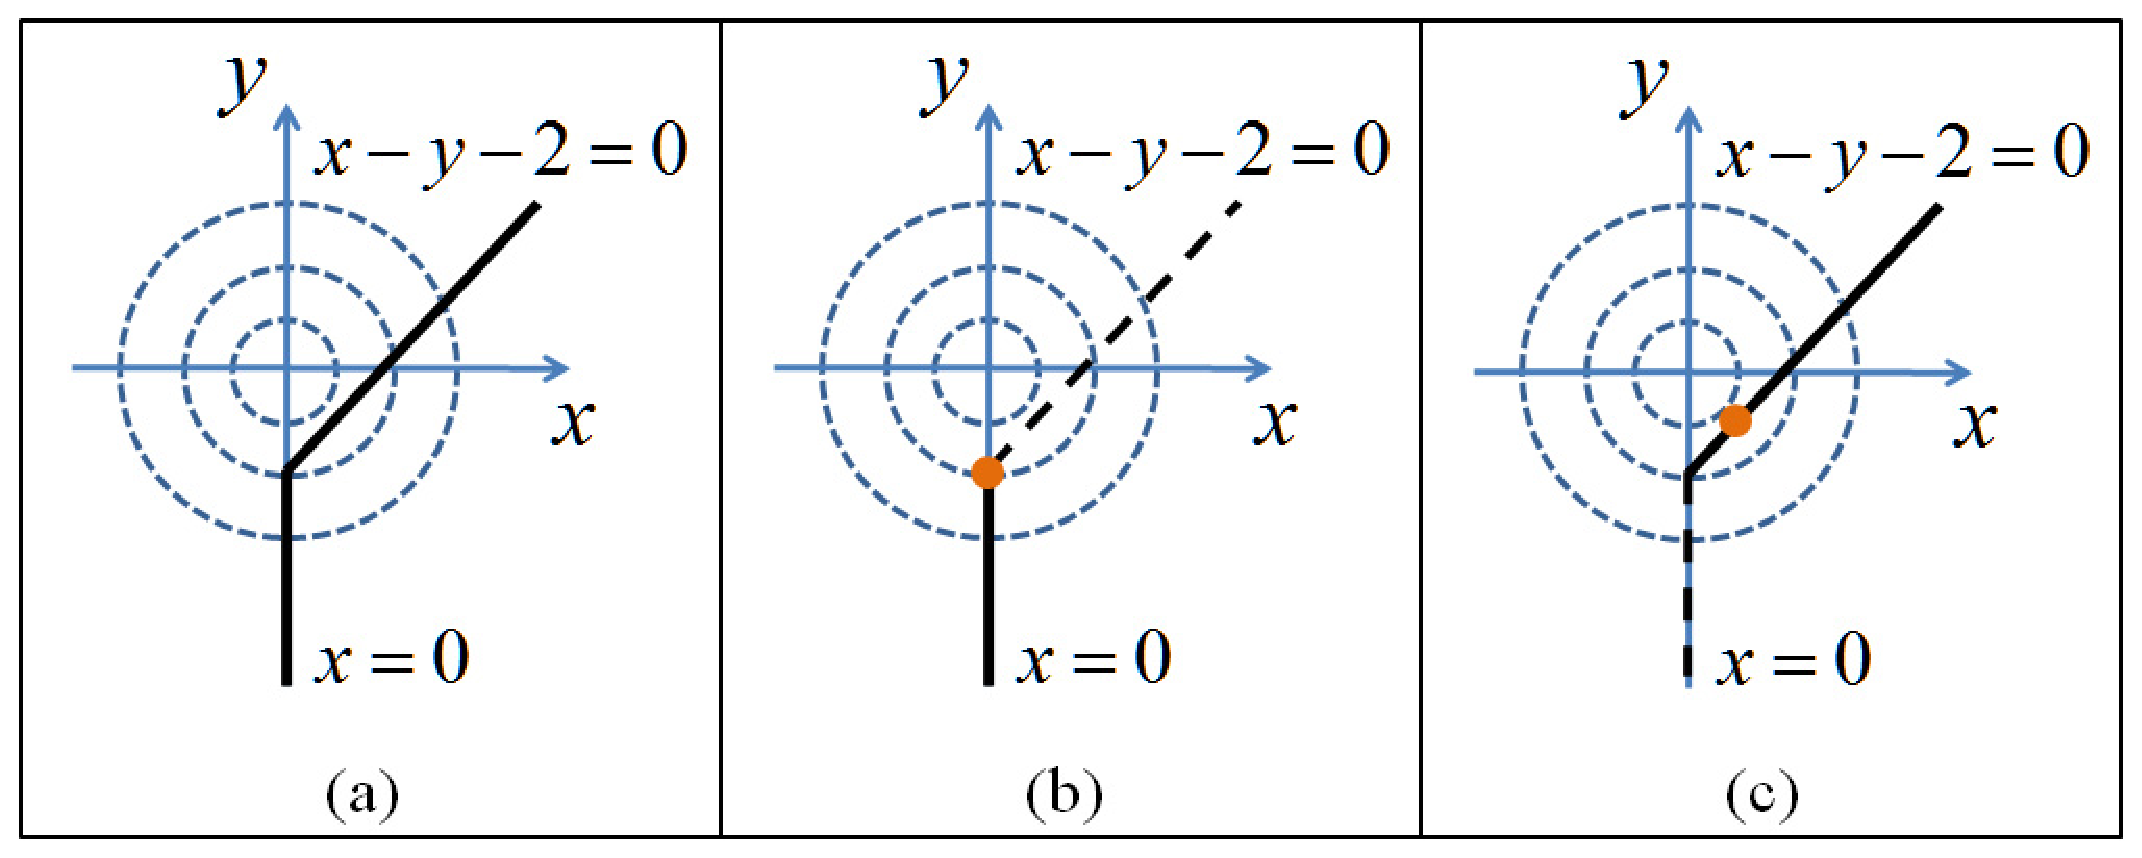
\includegraphics[width=5in]{figures/QPCC.eps}
  \caption{A simple 2D QPCC example. The complementarity constraints are $0\leq x \perp x-y-2 \geq 0$. (a) The feasible region lies in two intersecting half-hyperplanes, shown as two black line segments. (b) With the initial guess of $x=0$ and $x-y-2\geq 0$, the minimizer, shown as an orange dot, is located at the boundary of the inequality constraint. (c) After pivoting the constraint, setting $x\geq 0$ and $x-y-2=0$, we find a better minimizer (global minimizer in this simple case).}
  \label{fig:QPCC}
\end{figure}

Our algorithm further exploits the structure of a contact problem to
improve the performance. Instead of arbitrarily selecting a candidate
to pivot, we can group the complementarity constraints according to
their physical meaning and pivot a whole group together. There are
three different situations for each contact point: static, sliding and
contact breakage. Pivoting constraints in eq.
(\ref{eqn:initialGuess1}) indicates a switch between a static (or a
sliding) contact and contact breakage.  Pivoting constraints in
eq. (\ref{eqn:initialGuess2}) and (\ref{eqn:initialGuess3})
indicates a switch between static and sliding contact. For example, if
$\vc{f}_{\perp}(i)=0$ is the result of solving the QP (eq.
(\ref{eqn:initialGuess})), it implies that breaking $i$th contact point
might lead to a better minimizer for the QPCC. The solver will pivot
the corresponding constraints: $\vc{f}_{\perp}(i) \geq 0 \rightarrow
\vc{f}_{\perp}(i) = 0$ and $(\vc{N}^T\dot{\vc{p}}^{n+1})(i) = 0
\rightarrow (\vc{N}^T\dot{\vc{p}}^{n+1})(i) \geq 0$. The new QP will
be solved subsequently. Conversely, when a free point restores a static
contact, we apply the opposite pivoting.

If a friction cone condition (eq. (\ref{eqn:initialGuess3})) for the
$i$th contact point needs to be pivoted, this implies that the $i$th contact point is about to slide and switching it from static to sliding might lead to a better minimizer. The solver then changes the inequality constraint $(\mu \vc{f}_{\perp} - \vc{E}^T \vc{f}_{\parallel})(i)\geq 0$ to equality and changes the corresponding equality constraint $\lambda(i)=0$ to inequality. In addition, we need to pivot some constraints in eq. (\ref{eqn:initialGuess2}) to specify the direction of the sliding contact, which can be estimated using the static friction from the current minimizer. We project this static friction force to each of the tangential direction of the $i$th contact point $\vc{D}(i)$ and find the two directions (the $m$th and $n$th direction in $\vc{D}(i)$) that have the largest magnitude. The sliding force direction is estimated to be along the convex combination of $m$th and $n$th directions. We pivot the constraints in the following way,
\begin{align}
& \vc{f}_{\parallel}(i, m)\geq 0, \;\;\; (\vc{D}^T \dot{\vc{p}}^{n+1} + \vc{E} \lambda)(i, m) = 0 \nonumber \\
& \vc{f}_{\parallel}(i, n)\geq 0, \;\;\; (\vc{D}^T \dot{\vc{p}}^{n+1} + \vc{E} \lambda)(i, n) = 0\nonumber \\
& \vc{f}_{\parallel}(i, j) = 0, \;\;\;(\vc{D}^T \dot{\vc{p}}^{n+1} + \vc{E} \lambda)(i, j) \geq 0, ~~\forall j \neq m, n\nonumber
%(\vc{D}^T \dot{\vc{p}}^{n+1} + \vc{E} \lambda)(i, m) = 0 &
%(\vc{D}^T \dot{\vc{p}}^{n+1} + \vc{E} \lambda)(i, n) = 0 & \nonumber \\
%(\vc{D}^T \dot{\vc{p}}^{n+1} + \vc{E} \lambda)(i, j) \geq 0, & ~~\forall j \neq m, n \nonumber\\
\label{eqn:staticSlidePivot}
\end{align}
where $\vc{f}_{\parallel}(i, j)$ is the magnitude of the friction force
along the $j$th direction for the $i$th contact
point\footnote{$\vc{f}_{\parallel}(i, j)$ is actually the $(i\cdot N+j)$th
element of $\vc{f}_{\parallel}$ assuming that $N$ tangential directions
are used for the linearized friction cone for each contact point.}. For
the special case, where the friction force is exactly along the $m$th (or
$n$th) direction, we only pivot the complementarity constraints involving
the $m$th (or $n$th) direction. For a switch between sliding to static
contact, we use the same pivoting mechanism but pivot the constraints the
opposite way.

Instead of searching exhaustively in the feasible region of the QPCC, our
solver systematically explores the feasible region based on the above
mentioned heuristics. Although the objective value is not guaranteed to
decrease monotonically, our experiments show that the objective value
decreases drastically within a small number of iterations. The minimizer
found by our solver is, in all the experiments, significantly closer to
optimal than the one solved under the static contact assumption. We report the
results of the experiments in Chapter \ref{sec:softEvaluation}.

\paragraph{Implementation.}
Our solver requires a feasible initial guess. We can use the trivial solution under static contact assumption (eq. (\ref{eqn:initialGuess})) as an initial guess, or the solution from the previous QPCC when it is available (warm start). Occasionally, they might result in an infeasible QP. For those cases, we assume the same muscle activation as in last time step, remove the objective function and muscle length constraints from eq. (\ref{eqn:softOptimization}) and solve a pure LCP. The contact situation from the LCP solution is then used as the initial guess for the QPCC.

We implement the QPCC solver using a graph expansion algorithm (See Appendix \ref{chapter:AppendixA} for details). Each
QP with linear constraints is a node in the graph. We visit each node
twice, starting from the initial guess as the root. In the first
visit, we solve the QP, assign the objective value to the
node, and store the set of candidates to be pivoted. After first
visit, we push the node into a priority queue based on its objective
function value. A node is visited the second time when it is at the
top of the queue. In the second visit, we pivot the constraints from
its candidate set. Each pivot generates a child node. We discard the
child node if it already exists in the current graph. If the child
node is new, we visit the node for the first time and push it into the
queue. The second visit is completed when all the constraints in the
candidate set are pivoted. We then pop the next node in the queue and
repeat this process. The algorithm terminates when the priority queue
is empty or the number of visited nodes exceeds a threshold. The final
solution is the best minimizer found so far by the QPCC solver.

\section{Results}

\label{sec:softResults}
\begin{figure*}[ht]
\centering
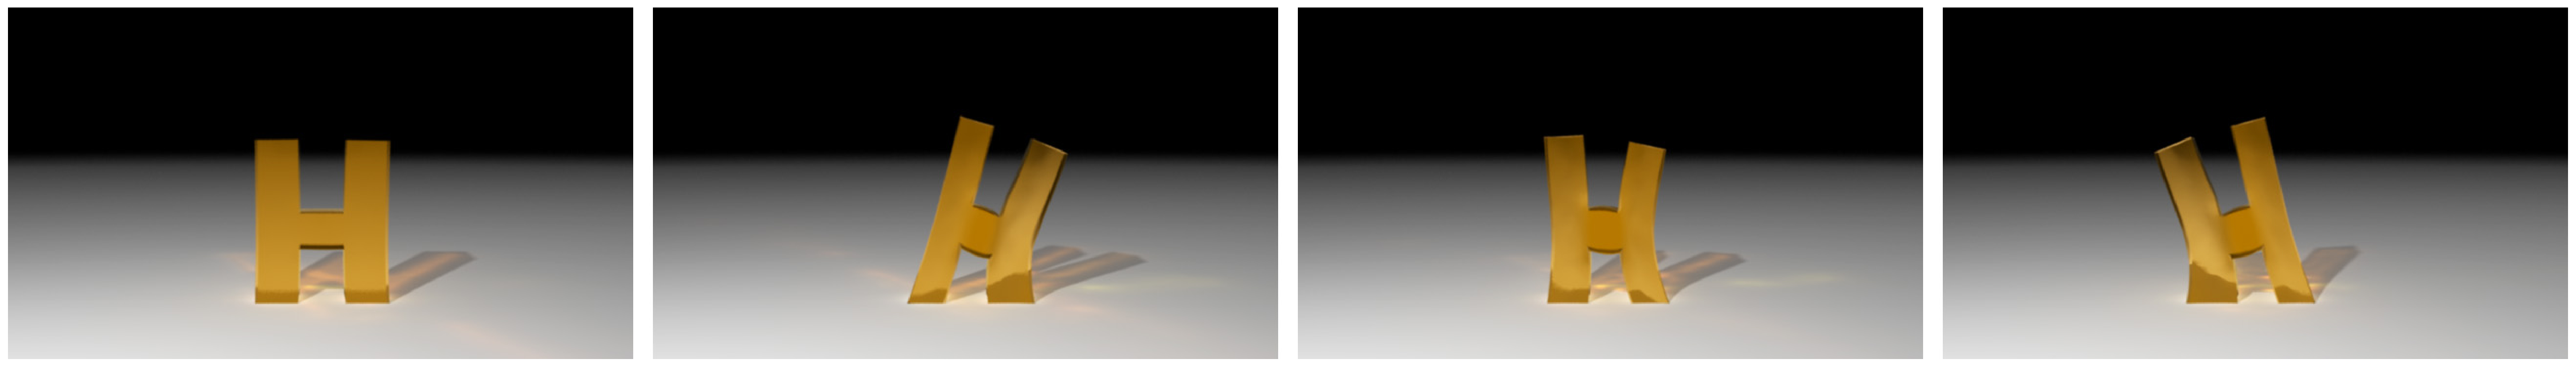
\includegraphics[width=\textwidth]{figures/HSwing.eps}
\caption{An H-shaped soft body character does its morning exercises by swinging its body from one side to the other.}
\label{fig:HSwing}
\end{figure*}

\begin{figure*}[ht]
\centering
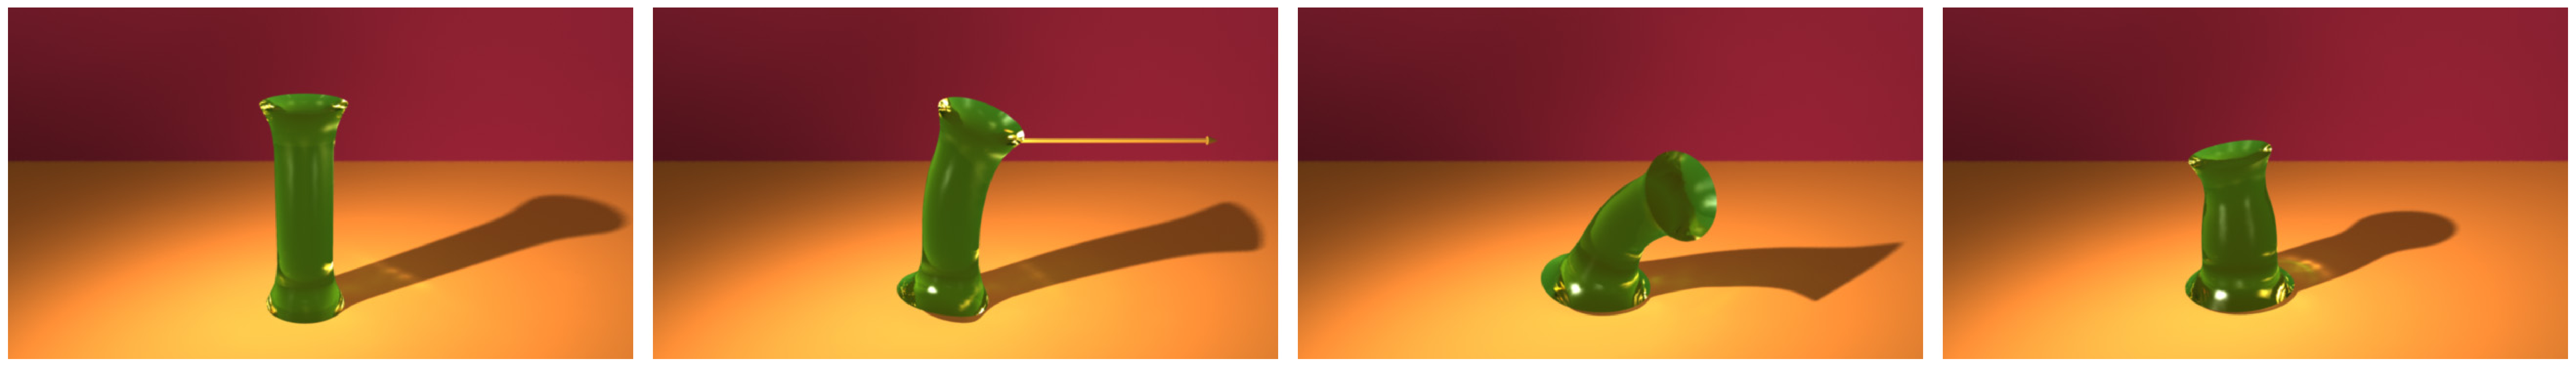
\includegraphics[width=\textwidth]{figures/IBalance.eps}
\caption{An I-shaped soft body character tries to maintain balance under
perturbation by regulating its momenta, widening its base and lowering its center of mass.}
\label{fig:IBalance}
\end{figure*}

In this section we describe the results of our soft body locomotion
controllers. Please see the video\footnote{http://dl.dropbox.com/u/36899427/softbodylocomotion.mp4} to watch the locomotion
animations. Our system is implemented in C++, and we generated the
tetrahedral mesh for FEM simulation using TETGEN \cite{Si:2006}. We
used the GPU to create layered depth figures for collision detection,
and we used contact patches (multi-resolution volume contact)
\cite{Allard:2010} instead of points as the contact primitives. For
each contact patch, we use eight tangential directions to linearize
the friction cone, which provides sufficient accuracy while keeping the QPCC tractable. The examples were run on a workstation with a
2.26GHz CPU and 4GB of memory. All the data of our locomotion
examples are summarized in Table~\ref{table:data}.

\begin{table}[!b]
  \centering
   \caption{Parameters and performance of examples. \# tets: the number of
  elements in the FEM simulation. \# dofs: the number of muscle degrees of
  freedom for the soft body. Sim time, opt time and total time are the average simulation,
  optimization and total time (in second) per frame.}
\begin{tabular}{|c|c|c|c|c|c|c|}
\hline
examples & \# tets & \# dofs  & \# contact     & sim  & opt & total\\
         & & & patches & time & time & time\\
 \hline
exercise(H) & 1901 & 52  & 4 & 0.54 & 0.05 & 0.59\\
balance(I)  & 1066 & 48  & 4 & 0.31 & 0.28 & 0.59\\
slide(F)    & 705  & 48  & 4 & 0.25 & 0.23 & 0.48 \\
jump(I)     & 1066 & 104 & 4 & 0.33 & 0.48 & 0.81 \\
jump(T)     & 1219 & 51  & 4 & 0.63 & 0.30 & 0.93 \\
roll(O)     & 911  & 40  & 6 & 0.26 & 0.18 & 0.44\\
crawl(I)    & 620  & 26  & 8 & 0.18 & 0.24 & 0.42\\
walk(X)     & 1128 & 112 & 4 & 0.54 & 0.70 & 1.24\\
\hline
 \end{tabular}
 \label{table:data}
 \end{table}

We design many different shapes of the soft body characters, all of
which are chosen from the English alphabet. Figure~\ref{fig:HSwing} shows
an H-shaped character doing morning exercises. The character is designed
with four longitudinal muscles and one radial muscle for each
leg (Figure~\ref{fig:muscles}a). It is animated by specifying the
trajectory of the desired center of mass (COM), which is moved left/right
by a sine function. We use the position and velocity tracking controller
from Chapter \ref{sec:controller} to track the desired COM. Note that when
the ``H'' swings left, its right side elongates and gets thinner while the
left side shortens and becomes fatter due to the volume preservation. This
animation clearly exemplifies the principle of \emph{squash and stretch}.

\paragraph{Balance.} We design an I-shaped character
(Figure~\ref{fig:IBalance}) to demonstrate static balance.  We gave
the character four longitudinal muscles that allow it to bend in any
direction.
This character is perturbed by a large force exerting at
its head, and it attempts to recover its balance. Static balance of
the ``I'' turns out to be one of the most difficult task among all our
examples. The geometry of the letter ``I'' does not have limbs or
other appendages to help it regulate the linear and angular
momentum. The squishy body and lack of skeletal support make the task
even more challenging. In addition to momentum control for balance,
which is not enough to prevent the ``I'' from falling, we exploit the
advantage of its flexible body shape.  We include a term in the
objective function that encourages it to widen its support base.  With
this wider base, the contact area is increased and the COM is lowered,
which helps with the balance task. Without our QPCC solver, base widening would be difficult
to achieve, because it requires frequent switching from static to sliding contacts.
In addition, we observe that right
after the perturbation, half of the base is lifted from the ground and
the contact area concentrates on the rim of the base to provide the maximum
amount of angular momentum to combat the perturbation. It is similar
to a human lifting his or her heels and using only toes to balance
when pushed from behind. This natural contact strategy
emerges automatically from our QPCC solution.  To compare our
QPCC solver and a more commonly used QP solver with linear
constraints, we produced two animation sequences of the ``I''
balancing, one with each solver.  QPCC produced natural and effective
balance motions, including changing contact situation, lowering the
COM, widening the base and regulating momentum. In contrast, the QP
solver (which only allows for static contact constraints) resulted in a falling motion.

\begin{figure*}[t]
\centering
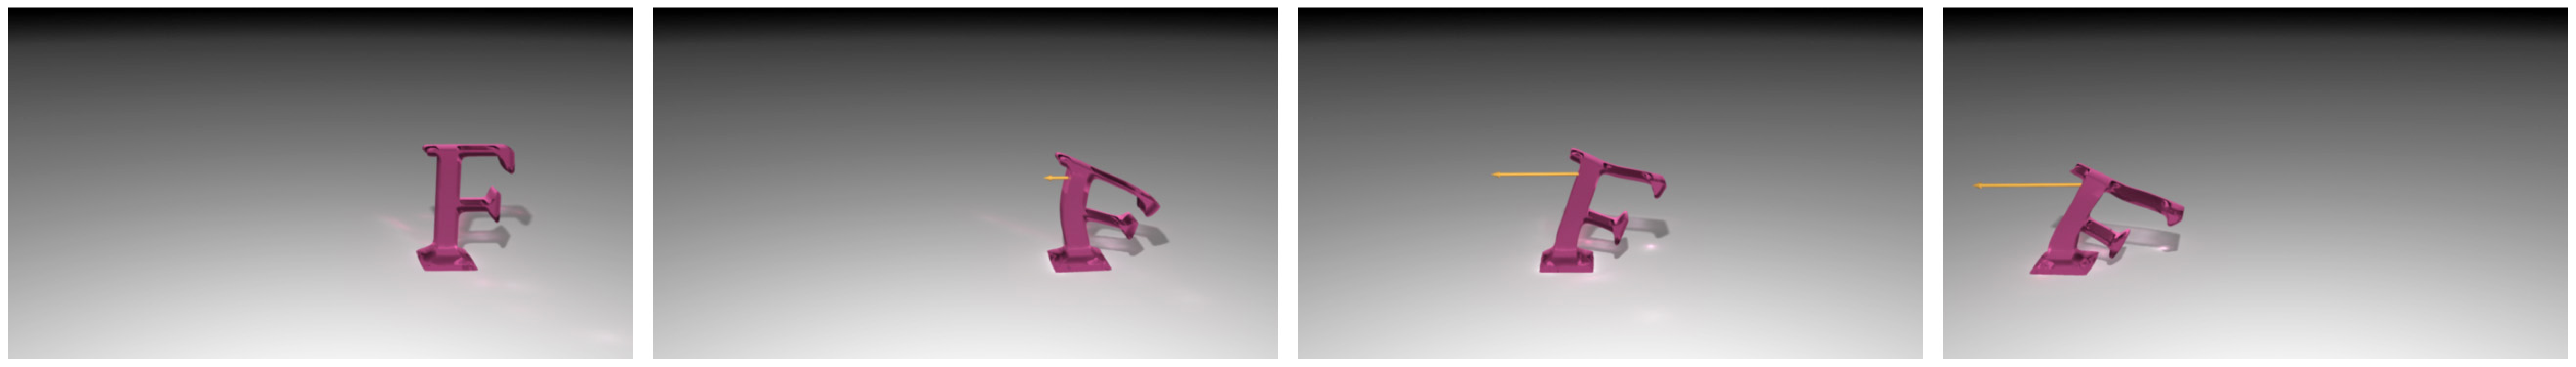
\includegraphics[width=\textwidth]{figures/FBalance.eps}
\caption{An F-shaped soft body character maintains balance under a persistent and continuously increasing pulling force on a slippery surface. It actively leans backward to avoid tipping over.}
\label{fig:FBalance}
\end{figure*}

\begin{figure*}[t]
\centering

\includegraphics[width=\textwidth]{figures/IJump.eps}
\caption{An I-shaped soft body character squashes and stretches its whole body to jump forward.}
\label{fig:IJump}
\end{figure*}


\paragraph{Sliding.} In the example of Figure~\ref{fig:FBalance},
instead of applying a perturbation force that lasts for a short time,
we exert an continuously increasing pulling force on the ``F'' standing on
a slippery surface. We design a sliding balance controller for this
special balance task. The controller estimates the optimal relative
position between the center of base (COB) and the COM such that the
total angular momentum is zero. We use the position and tracking controller to track the optimal COB. The sliding balance controller also benefits from our QPCC
solution since planning the movement of the COB involves planing the
change of contact situation (from static to sliding).  We instrument the vertical stroke of the ``F'' with four
longitudinal muscles. Even though no muscle resides in the horizontal
parts of this character, the two horizontal strokes are still
influenced by the muscles in the main body. The first sequence of
sliding balance in the video shows that the ``F'' leans left while it is
dragged towards the right.  As the drag force increases, the ``F'' leans more
and more to prevent from tipping over. The second sequence shows the
sliding motion when it is dragged to the left. The sliding motion is
different from the first one due to the asymmetry of the body
shape. The elongation and oscillation of the top stroke of the ``F''
demonstrates the animation principle of \emph{follow through}. In the
third sequence, we applied the sliding balance controller 0.3 second
after the start of dragging to delay the character's
response time. The slow response of the ``F'' makes it difficult to
maintain the optimal COB-COM relative position. It struggles to keep
balance by constantly switching between sliding and breaking contact
(small jumps), and eventually it manages to balance.  These changes of
contact, due to the QPCC solver, makes the controller more robust and
the soft body character more lifelike.

\begin{figure*}[t]
\centering
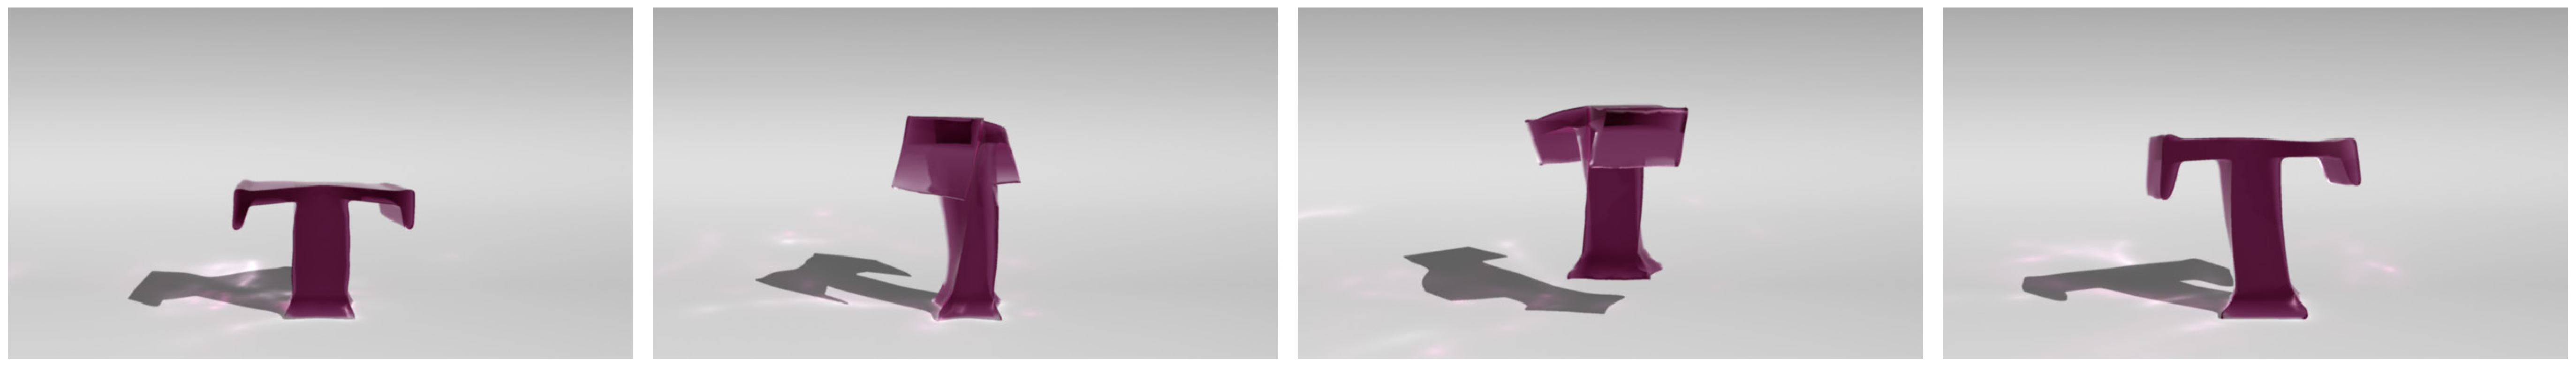
\includegraphics[width=\textwidth]{figures/TTwist.eps}
\caption{A T-shaped soft body character twists using helical muscles when jumping.}
\label{fig:TJump}
\end{figure*}

\begin{figure*}[t]
\centering
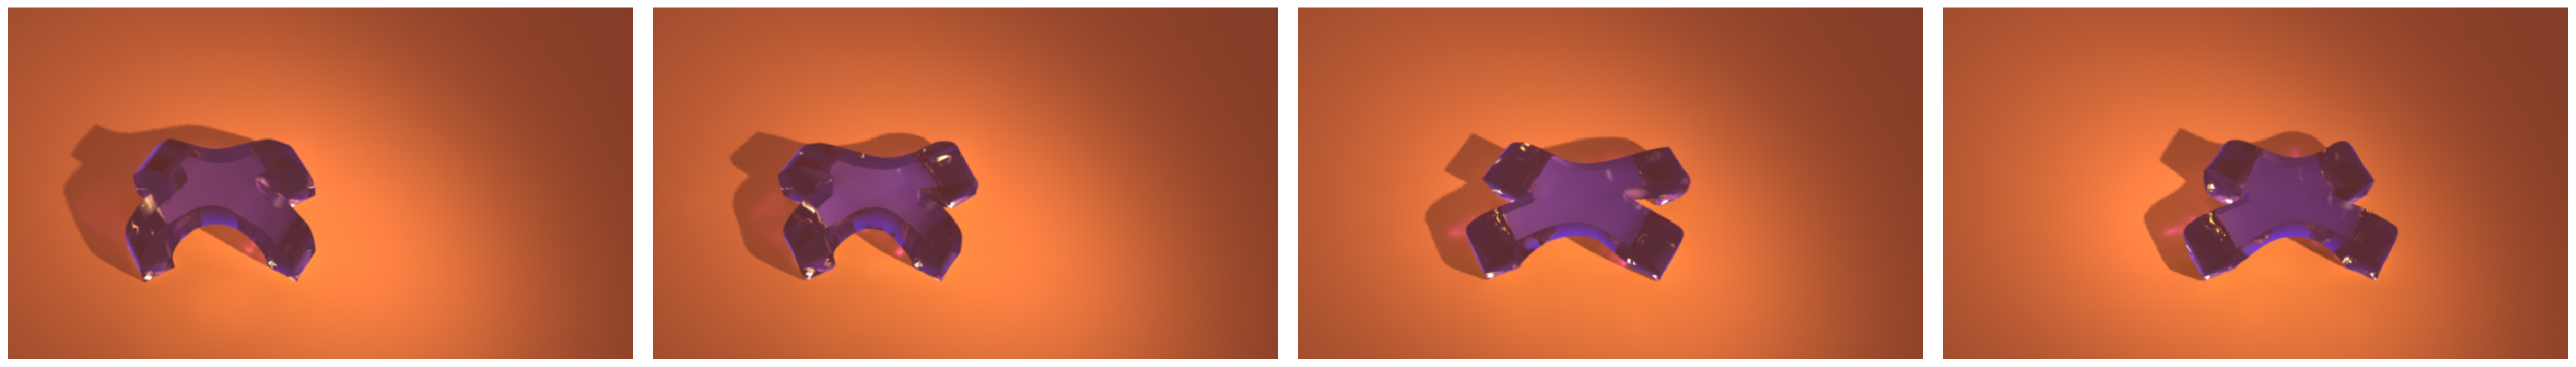
\includegraphics[width=\textwidth]{figures/XWalk.eps}
\caption{An X-shaped soft body quadraped walks by slowly lifting and moving one foot at a time.}
\label{fig:XWalk}
\end{figure*}


\begin{figure}[!b]
\centering
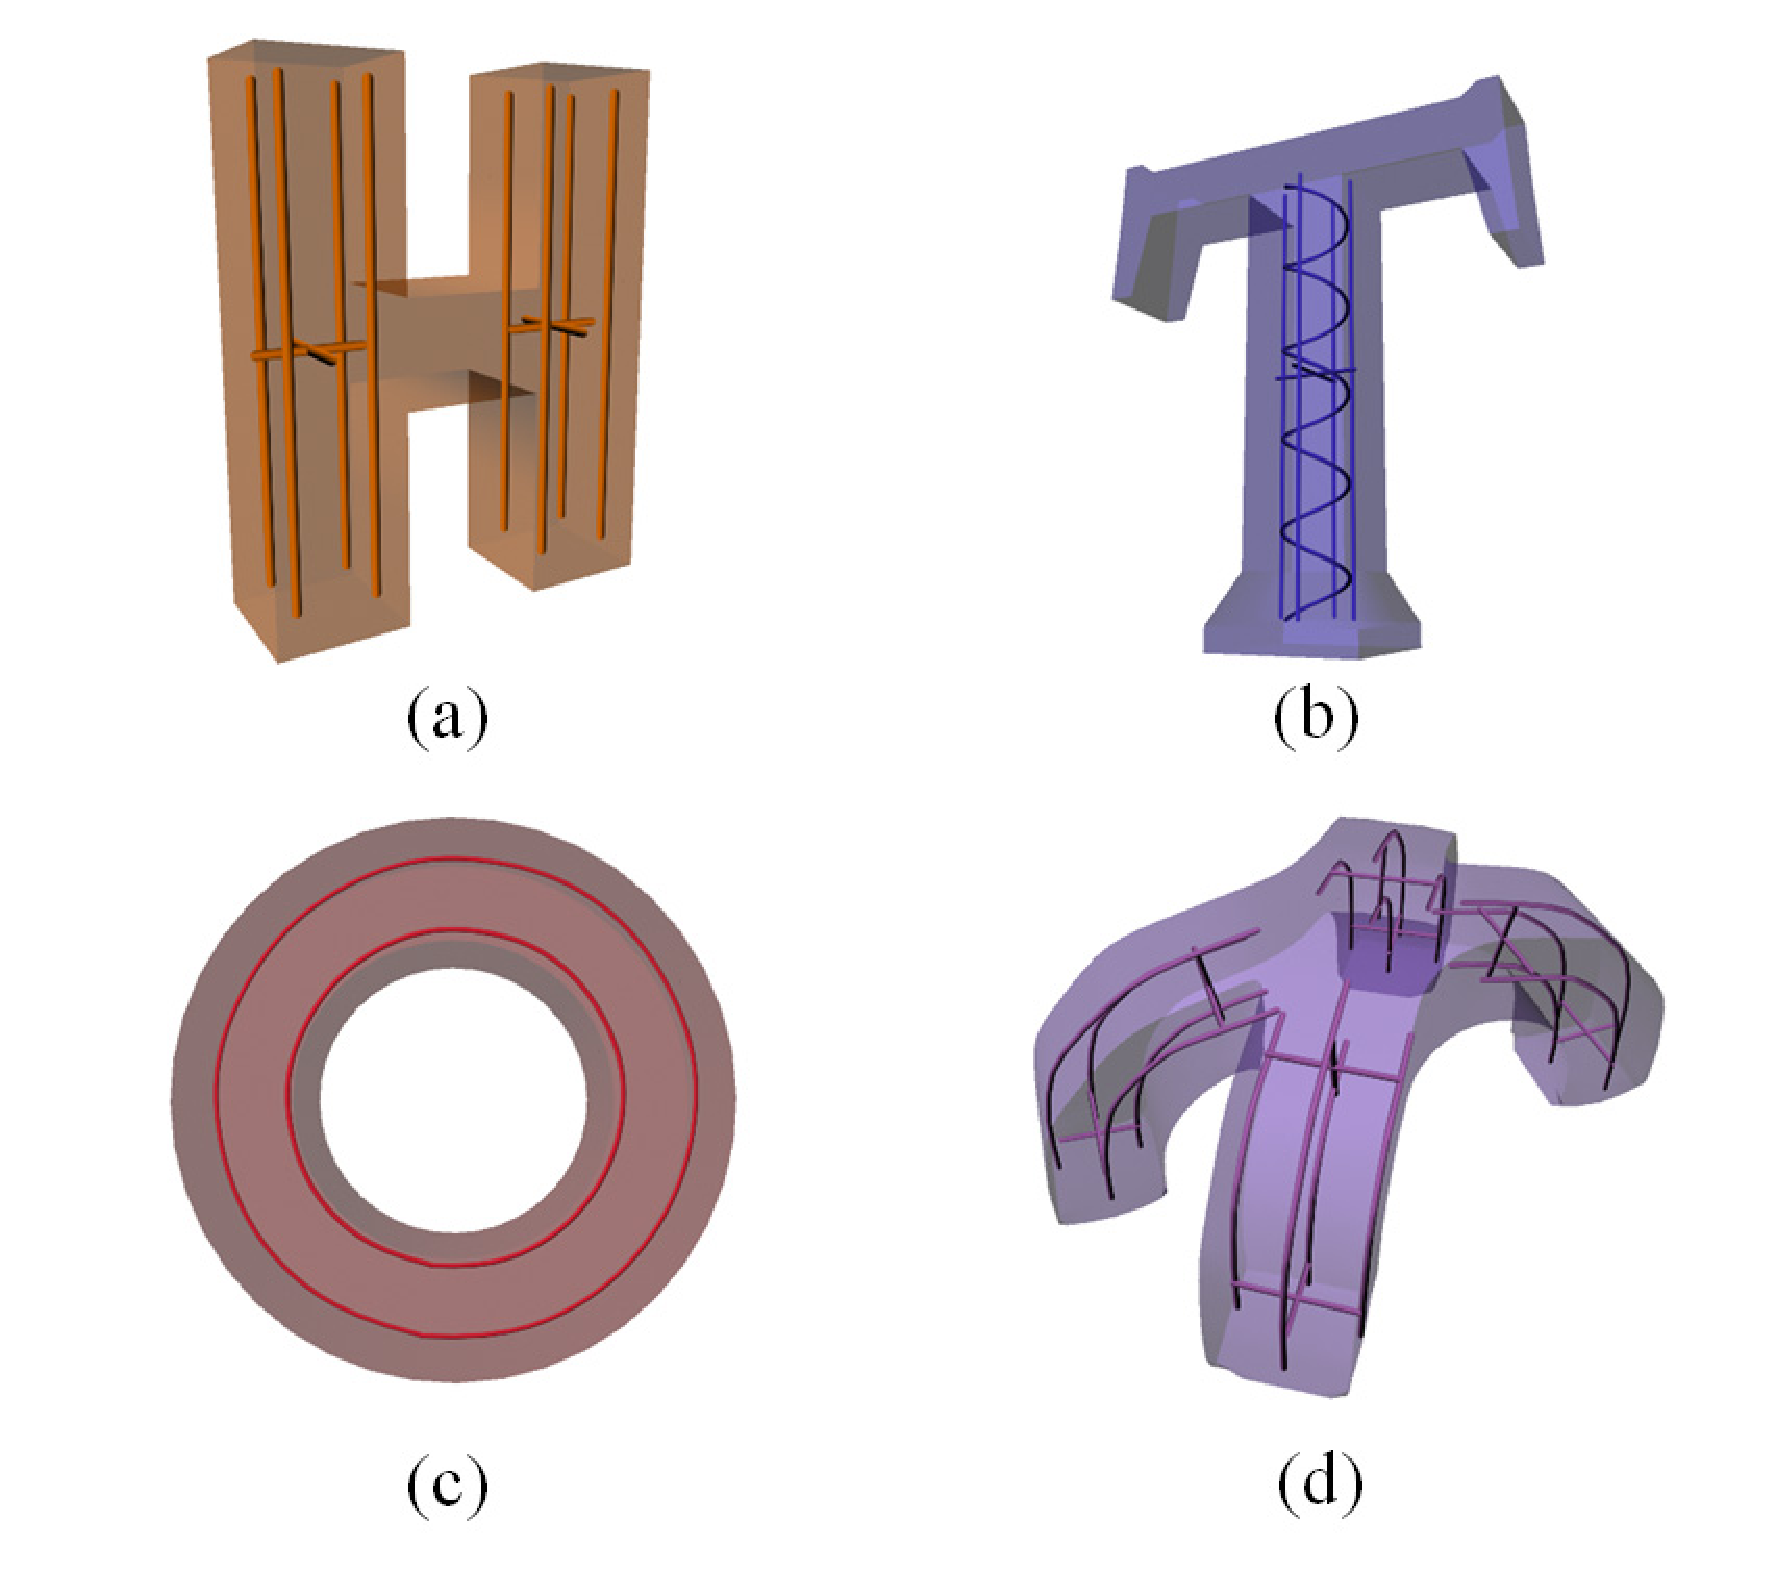
\includegraphics[width=3in]{figures/muscles2.eps}
\caption{Examples of the muscle fiber designs for various soft body characters. Each curve inside the character represents a muscle fiber, which consists of a number of independently contracting degrees of freedom.}
\label{fig:muscles}
\end{figure}

\paragraph{Jumping.} Jumping is an visually interesting form of
locomotion for soft body characters as it is often seen in cartoons
and animations. Our jumping controller consists of three separate
controllers for takeoff phase, airborne phase, and landing
phase. During the takeoff phase, we use the position and velocity
tracking controller to follow a desired trajectory of the COM. We also
set $\bar{\dot{H}}=\vc{0}$ to the angular momentum controller, which
prevents large rotation at takeoff.  During the airborne phase, we control the relative
position between the COB and COM. Extending the COB towards the
direction of jumping helps the character balance after landing. Upon
landing, we switch to the static balance controller.
Figure~\ref{fig:IJump} shows a forward jumping motion of the same
character ``I'' with a slightly different fiber arrangement.
We add four more longitudinal muscles and one radial muscle to help it with this highly dynamic motion.
Another sequence in the video shows successive jumps in place.
Figure~\ref{fig:TJump} demonstrates
a twist jump and the use of helical muscles
(Figure~\ref{fig:muscles}b).  Before the ``T'' takes off, we set
$\bar{\dot{H}}=(0, 600, 0)^T$ to make it twist its body.

\paragraph{Rolling.} In the video, we also demonstrate
locomotion by rolling. We designed an O-shaped character with two
loops of muscle fibers arranged as two concentric circles
(Figure~\ref{fig:muscles}c). Each fiber consists of 20 independent segments, which allow
the ``O'' to control its shape locally. The rolling motion is initiated by moving the COM in front of the contact patches. We use the angular momentum control to
make it roll. In the first animation, we set the desired
change of angular momentum $\bar{\dot{H}}$ to be $(0, 0, -200)^T$ in
the first 90 frames. We observe that the character actively changes its
shape by shifting its weight to the right in order to roll. After the character starts rolling,
we disable the controller
and simulate the passive rolling. The character recovers to its
original symmetric rounded shape and the rolling stops after a while
due to friction. In the second animation, we compare our result with
the motion solved by a QP using the static contact assumption.  When we only
allow static contact, the ``O'' never begins rolling because this
motion requires the character to break contact, which is prohibited by the static contact assumption (eq.~(\ref{eqn:initialGuess1})).  The third sequence
shows that the ``O'' starts to roll right, deaccelerates, stops
and rolls to the left by applying a time varying $\bar{\dot{H}}$ to
the controller.

\paragraph{Crawling.} Crawling is often used by soft body creatures in
nature, such as earthworms.  To demonstrate crawling motion, we
flatten the ``I'' and lay it down on the ground. In addition to the
four longitudinal muscles run along four sides of the body, we add
another radial muscle in the middle of its body to facilitate the
elongation of the body. We specify the trajectory of its four
corners for the crawling motion; the back of the character moves while
it is contracting, and the front moves when it elongates.  We use the
position and velocity tracking controllers to match the trajectory. As
Miller noted, such creatures have oriented scales that result in
anisotropic friction~\cite{Miller:1988}.  We incorporate just such an
anisotropic friction into our contact model by modifying the contact
force to $\vc{f}_c=\vc{N}f_\perp+\vc{DS}\vc{f}_\parallel$, where
$\vc{S}$ is a diagonal scaling matrix that modulates the frictional
force according to the direction of motion. We set the friction
coefficient in the backward direction to be 10 times larger than all
other directions. In the video, we demonstrate the
earthworm style of crawling. The whole body of the character lies flat
on the ground at all times and it moves forward by repeatedly
shortening and elongating its body. The contact strategy of this form
of crawling is complex. During shortening, the front end of the body
is in static contact while the rear end is sliding forward. During
elongating, the front end switches to sliding contact while the rear
end switches to static contact. It is challenge to capture this
complex contact strategy using the traditional control mechanism, but
it emerges automatically by solving QPCC.

We also demonstrates an inchworm style of crawling, using the same
body geometry and muscles as the earthworm. For this style of motion,
the body bends upward periodically at the middle and the contacts
mostly concentrate at the two ends of the body. We achieve this effect
using the same controller as in the earthworm style crawling with an
additional constraint that the upper longitudinal muscle cannot
contract.  While other muscles contract to tracking the trajectory,
the asymmetric muscle contractions bend the body upwards naturally.

\paragraph{Walking.} Figure~\ref{fig:XWalk} demonstrates the walking
motion of an X-shaped quadruped. We instrument four longitudinal
muscles and two radial muscles for each limb of the ``X''
(Figure~\ref{fig:muscles}d) and specify the trajectories for all of
its four feet. We apply the position and velocity tracking controller, to track this the walking motion.
The first sequence in the video shows a careful and slow gait that moves only one
foot at a time. The second walking sequence shows a faster walking
gait by simultaneously lifting and moving two feet at a time. The
breaking of contact when a foot lifts from the ground is handled
automatically by the QPCC solver.

\section{Discussion}
\label{sec:softEvaluation}

We have presented a system for animating soft body characters, with a
particular emphasis on locomotion.  Key aspects of our approach include
the coordinated deformation of groups of finite elements using virtual
muscle fibers, the specification of high-level goals by the animator, and
the use of a new solver that handles static, sliding and breaking contact
cases.  Our system allows us to create soft body characters that
demonstrate a variety of locomotion behaviors, including crawling,
hopping, walking, sliding and rolling.  Our characters move in an organic
manner, and they follow the animation principles of anticipation,
squash-and-stretch, and follow through.

One important contribution of this chapter is the formulation of QPCC and its solver.
QPCC is an NP-hard problem \cite{Braun:2005} and our method provides an effective heuristic.
To evaluate our QPCC solver, we tested it on $10$
QPCC problems with 98 variables and 40 pairs of linear complementarity
constraints. We compared our solutions (QPCC in Table~\ref{tab:qpcc}) with the ground truth, as well
as with the solutions based on the static contact assumption (QP in Table~\ref{tab:qpcc}). The
ground truth is computed by an exhaustive search, \ie, solving a QP
for every combination of complementarity variables and selecting the one
with the lowest objective value. We evaluated our results using a ``gap
ratio'', defined as the ratio of difference in the optimal value between
our solver and the ground truth, to the difference in the optimal value
between the static contact assumption and the ground truth. On average
of $10$ problems, the gap ratio is $6.29$, indicating that our solver
yields solutions $6.29$ times closer to the ground truth than the
solutions based static contact assumption. We also selected the best
case and the worst case according to the gap ratio and reported them
in Table \ref{tab:qpcc}.
\begin{table*}
  \centering
   \caption{The results of the numerical experiments of the QPCC solver. }
\begin{tabular}{|l|r|r|r|r|r|r|r|r|r|r|}
\hline
&\multicolumn{3}{|c|}{QPCC} & \multicolumn{3}{|c|}{QP}  & \multicolumn{3}{|c|}{Ground Truth} \\ \hline
& Avg & Best & Worst & Avg & Best & Worst & Avg & Best & Worst \\ \hline
Obj Value & 1483.2 & 21.8 & 697.9 & 5222.8 & 2072.0& 1246.9 & 772.9 & 0.0 & 0.0 \\ \hline
\#Iterations & 17 & 3 & 31 & 1 & 1 & 1 & 10000 & 10000 & 10000 \\
\hline
\end{tabular}
 \label{tab:qpcc}
\end{table*}
Although the empirical results showed that our QPCC solver can
effectively solve contact resolution problem and balance between the
quality of solution and computational time, the QPCC solver does not
guarantee finding the minimizer in polynomial time. In the
worst case, it takes the same amount of time as the exhaustive search
to find the global minimizer.

Our system has a few limitations.  The
optimization scheme described in Chapter \ref{sec:softControl} only
optimizes the control variables for the next time step. This type of
greedy algorithm sometimes leads to unnaturally large muscle contraction or
discontinuities in motion. For example, the rolling ``O'' demo in the
video exhibits some unnatural vibration. Furthermore, the greedy algorithm prevents us
from simulating anticipatory behaviors in motion. For example, we were
not able to develop a ``cartwheel'' controller for the I-shaped
character because a natural and stable cartwheel motion requires
optimizing a long-window of trajectory. This issue can potentially be
solved by implementing long-horizon optimization or model predictive
control methods.

One of the issues that we hope to explore in the future is to expand
our solution techniques to handle longer-term goals that cannot be
reached using our current optimization method. In this work, all muscles are manually designed. We would like to develop an automatic muscle design algorithm to incorporate more sophisticated muscle structures.
We would also like to
investigate muscle design for chunkier creatures. For example, it is
not immediately obvious how muscle fibers should be arranged for the
Stanford Bunny. Another possibility is to note that in our current
system, we only use contracting muscle fibers in order to change the
shape of our characters.  It would be interesting to explore other
forms of shape control, such as elongating muscles or sheets of
virtual muscles.  Another possible direction would be to explore the
animation of soft body characters in water, since many real soft-body
creatures live in an aquatic environment.  Finally, our current
animator controls are provided as program modules, and an easier way
to use them would be to plug them together using a graphical user
interface.
